\subsection{Address Spaces}
\label{sec:address_spaces}

While performing computation, an Intel processor moves data between four
distinct physical address spaces, shown in Figure~\ref{fig:address_spaces}. The
address spaces overlap partially, in both purpose and contents, which can lead
to confusion. This section gives a high-level overview of the physical address
spaces defined by the Intel architecture, with an emphasis on their purpose and
the methods used to manage them.

\begin{figure}[hbtp]
  \center{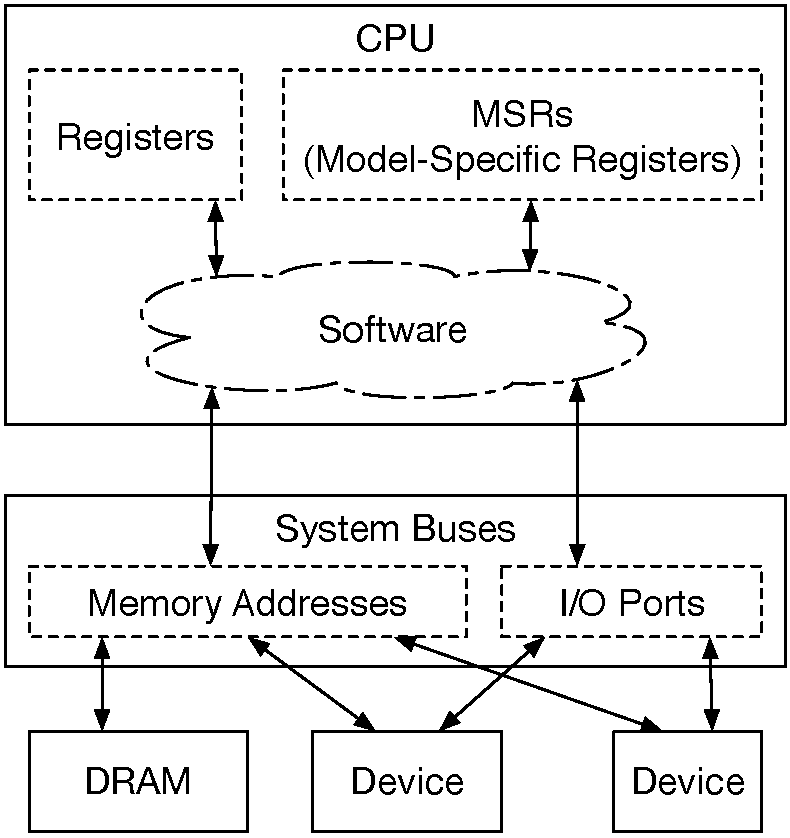
\includegraphics[width=55mm]{figures/address_spaces.pdf}}
  \caption{
    The four physical address spaces used by an Intel CPU. The registers and
    MSRs are internal to the CPU, while the memory and I/O address spaces are
    used to communicate with DRAM and other devices via system buses.
  }
  \label{fig:address_spaces}
\end{figure}

The \textit{register} space consists of names that are used to access the CPU's
register file, which is the only memory that operates at the CPU's clock
frequency and can be used without any latency penalty. The register space is
defined by the CPU's architecture, and documented in the SDM.

Some registers, such as the \textit{Control Registers} (CRs) play specific
roles in configuring the CPU's operation. For example, CR3 plays a central role
in address translation (\S~\ref{sec:paging}). These registers can only be
accessed by system software. The rest of the registers make up an application's
\textit{execution context} (\S~\ref{sec:registers}), which is essentially a
high-speed scratch space. These registers can by accessed at all privilege
levels, and their allocation is managed by the software's compiler. Many CPU
instructions only operate on data in registers, and only place their results in
registers.

The \textit{memory} space, generally referred to as \textit{the address space}
\textit{the physical address space}, consists of $2^{36}$ (64 GB) - $2^{40}$
(1 TB) addresses. The memory space is primarily used to access
\textit{Dynamic Random-Access Memory} (DRAM), the computer's main memory, but
it is also used to communicate with \textit{memory-mapped devices} that read
memory requests off a system bus and write replies for the CPU. Some CPU
instructions can read their inputs from the memory space, or store the results
using the memory space.

A better-known example of memory mapping is that at computer startup, memory
addresses 0xFFFFF000 - 0xFFFFFFFF (the 64 KB of memory right below the 4 GB
mark) are mapped to a flash memory device that holds the code for booting the
computer.

This memory space is partitioned between devices and DRAM by the computer's
firmware during the boot stage. Sometimes, system software includes
motherboard-specific code that modifies the memory space partitioning. The OS
kernel relies on address translation, described in \S~\ref{sec:paging}, to
control the applications' access to the memory space. The hypervisor relies on
the same mechanism to control the guest OSes.

% I/O Address Space: SDM vol1 S 16.3

The \textit{input/output} (I/O) space consists of $2^{16}$ I/O addresses,
usually called \textit{ports}. The I/O ports are used exclusively to
communicate with devices. The CPU provides specific instructions for reading
from and writing to the I/O space. I/O ports are allocated to devices by formal
or de-facto standards. For example, ports 0xCF8 and 0xCFC are always used to
access the PCI express (\S~\ref{sec:motherboard}) configuration space.

The CPU implements a mechanism for system software to provide fine-grained I/O
access to applications. However, all modern kernels restrict application
software from accessing the I/O space directly, in order to limit the damage
potential of application bugs.

% Architectural MSRs: SDM S 35.1
% Time-Stamp Counter: SDM S 17.13

The \textit{Model-Specific Register} (MSR) space consists of $2^{32}$ MSRs,
which are used to configure the CPU's operation. The MSR space was initially
intended for the use of CPU model-specific firmware, but some MSRs have been
promoted to \textit{architectural MSR} status, making their semantics a part of
the Intel architecture. For example, architectural MSR 0x10 holds a
high-resolution monotonically increasing time-stamp counter.

The CPU provides instructions for reading from and writing to the MSR space.
The instructions can only be used by system software. Some MSRs are also
exposed by instructions accessible to applications. For example, applications
can read the time-stamp counter with the \texttt{RDTSC} and \texttt{RDTSCP},
which are very useful for benchmarking and optimizing software, but also for
mounting timing attacks.
